\section{Introduction}
\label{intro}


\newcommand{\xidx}{i}
\newcommand{\yidx}{j}
\newcommand{\xw}[1]{w_{#1}}
\newcommand{\yw}[1]{w'_{#1}}

Dynamic Programming algorithms (DP) build optimal solutions to a problem by combining
together optimal solutions to many overlapping subproblems.  DP
algorithms exploit this overlap to explore otherwise exponential-sized
problem spaces in polynomial time, making them central to many
important applications ranging from logistics to computational
biology. A recent textbook \cite{DurbinEdKr98} on biological sequence analysis, for example,
lists 11 applications of DP in bioinformatics in its introductory
chapter with many more in chapters that follow.


Dynamic programs are usually described through recurrence relations
that specify how the cells in a DP table must be filled up
using solutions already computed for other cells, but recent research has shown that it is possible
to achieve order-of-magnitude performance improvements over this
standard implementation approach by developing \emph{divide-and-conquer}
 implementation strategies that recursively
partition the problem into smaller subproblems.  These strategies
exhibit better temporal locality, and the partitioning can expose more
optimization opportunities (see, e.g., \cite{IPDPS15/Tithi}). 
Even when compared with tiled implementations optimized by the best polyhedral compilers, 
the divide-and-conquer implementations still show significantly better performance, in some cases
by more than an order of magnitude as illustrated in \Cref{intro:performance}. 
\rch{Those plots appear in \cite{IPDPS15/Tithi}}
\asolar{write the previous  par a little differently to account for the recent publication}
Unfortunately, developing such implementations is quite difficult, as will become apparent in \Cref{divide}.
In this paper, we develop a new computer aided approach to formally deriving provably correct divide-and-conquer algorithms
for dynamic programming problems. The approach relies on a new method to formalize the derivation of these algorithms, which
allows an algorithm designer to guide the derivation process through a small number of very high-level tactics. 
Specifically, our paper makes the following contributions:
\begin{enumerate}
  \item We develop a small set of formal tactics that can be used to transform a class of recurrence
  specifications, written in a simple functional language, 
  into equivalent divide-and-conquer programs, that admit parallel cache-local
  implementations, in a principled, systematic manner.
  \item We prove that these tactics are semantics-preserving, assuming some side conditions are met
  at the point when the tactic is applied.
  \item We show that the side conditions can be effectively translated into first-order closed
  formulas, and verified automatically by SMT solvers.
\end{enumerate}



\begin{figure*}
\resizebox{\textwidth}{!}{\begin{tikzpicture}[>=latex,mark options={scale=.5}]
	\begin{axis}[
	    ymode=log,
		xlabel=Problem size,
		ylabel=Time ({\it s}),
		scaled x ticks=false, %{real:1000}
		log basis y=2, ymajorgrids=true]
	\addplot[color=blue!50!white,ultra thick,mark=*,smooth] table[x=n/Time(s),y=COZ] {data/perf-gap.txt}
	  node(COZ-curve) [coordinate,pos=0.9] {};
	\addplot[color=orange!70!white,ultra thick,mark=*,smooth] table[x=n/Time(s),y=CO] {data/perf-gap.txt}
	  node(CO-curve) [coordinate,pos=0.8] {};
	\addplot[color=olive!70!white,ultra thick,mark=*,smooth] table[x=n/Time(s),y=LOOPDP] {data/perf-gap.txt}
	  [yshift=-12pt] node[pos=0.05] {LOOPDP};
	\addplot[color=red!70!white,ultra thick,mark=*,smooth] table[x=n/Time(s),y=Bellmania] {data/perf-gap.txt}
	  node(Bellmania-curve) [coordinate,pos=0.85] {};
	\end{axis}
	
	\begin{scope}[anchor=west]
	  \node(CO-lbl)[orange!80!white] at(2,1.5) {CO\_Opt};
	  \node(Bellmania-lbl)[red!80!white] at(1.5,1) {Bellmania};
	  \node(COZ-lbl)[blue!80!white] at(1.25,.5) {COZ};
	\end{scope}
	\begin{scope}[->,dashed]
	  \draw[orange] (CO-lbl) -- (CO-curve);
	  \draw[red] (Bellmania-lbl) -- (Bellmania-curve);
	  \draw[blue] (COZ-lbl) -- (COZ-curve);
	\end{scope}
\end{tikzpicture}

}
\caption{\label{intro:performance}
  Comparison of the the best performance obtained using polyhedral compilers 
  (PluTo\,\cite{HPC10/Pouchet}, PoCC\,\cite{PLDI08/Bondhugula})
  for parallelization, vs. manually crafted recursive divide-and-conquer implementations (CO),
  taken from~\cite{IPDPS15/Tithi}.}
\end{figure*}

\section{Divide and Conquer DP}
\label{divide}

As a motivating example, we consider the Simplified Arbiter problem.
Two processes $x$ and $y$ are scheduled to run $|x|$ and $|y|$ time slots,
respectively. Execution starts at $t=0$, and the length of each time slot is
one time unit. The cost for scheduling the slots $[i..p)$ of $x$ at $t=i+j$
is given by $\xw{ipj}$, and the cost for schedulting the slots $[j..q)$ of $y$
also at $t=i+j$ is given by $\yw{jqi}$. \rch{$[i..p)$ or $(p..i]$? $[j..q)$ or $(q..j]$?
$\xw{ipj}$ or $\xw{pij}$? $\yw{jqi}$ or $\yw{qji}$?}

\begin{figure}
\begin{tabular}{@{\hspace{-1pt}}r@{~}l@{}}
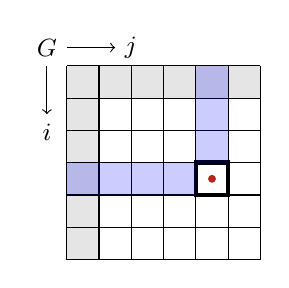
\begin{tikzpicture}[x=4.1mm,y=4.1mm,baseline=(center), remember picture]
  \coordinate(center) at (3,3);
  \draw[step=1] (0,0) grid (6,6);
  \draw[ultra thick] (4,2) rectangle +(1,1);
  %\node(Gij) at (4.5,2.5) {\tiny $\scriptscriptstyle\langle i,j\rangle$};
  \node[circle,fill=BrickRed,inner sep=0,minimum size=1mm](Gij) at (4.5,2.5) {};
  \fill[black,opacity=0.1] (0,5) rectangle (6,6);
  \fill[black,opacity=0.1] (0,0) rectangle (1,5);
  \fill[blue,opacity=0.2] (0,2) rectangle (4,3);
  \fill[blue,opacity=0.2] (4,3) rectangle (5,6);
  \node[anchor=south east](G) at (0,6) {\small$G$};
  \draw[->] (G.east) -- +(1.5,0) node[anchor=west] {\small $j$};
  \draw[->] (G.south) -- +(0,-1.5) node[anchor=north] {\small $i$};
\end{tikzpicture}
&
\small
$
\begin{array}{l@{}}
	\tikz[overlay, remember picture]{\draw[BrickRed] (0,0) -- (Gij);}
	G_{ij} ~=~ \\
	~
	\begin{cases}
		0                        & i=j=0 \\
		\yw{0j0}                  & i=0, j>0 \\
		\xw{0i0}                 & i>0, j=0 \\
		\begin{array}{@{}l@{\hspace{-1pt}}l@{\hspace{-4pt}}}
		  \min\langle & \underset{0\leq q<j}\min ~ G_{iq} + \yw{qji},  \\
		              & \underset{0\leq p<i}\min ~ G_{pj} + \xw{pij}~\rangle
		\end{array}              & i,j>0
	\end{cases}
\end{array}
$
\end{tabular}
\vspace{5pt}
\caption{Recurrence equation and cell-level dependencies.}
\label{intro:arbiter spec}
\end{figure}


The optimal cost for scheduling the first $i$ slots of $x$ and the first $j$ slots
of $y$ is given by the recurrence in \Cref{intro:arbiter spec}. When $i$ is zero, it means that
only $y$ has been scheduled, so the cost is $\yw{0j0}$, and similarly when $j$ is zero, 
the cost is $\xw{0i0}$. In the general case, either the schedule ends with time allocated to $x$, 
in which case $x$ was allocated time from some step $p$ to $i$, and the cost is 
$G_{pj} + \xw{pij}$, or the schedule ends with time allocated to $y$, in which case, 
$y$ was allocated time from some step $q$ to $j$, and the cost is $G_{iq} + \yw{qji}$.
In order to determine which is the case, and what is the optimal value of $p$ and $q$, 
the dynamic programming algorithm needs information from all cells above and to the left of $G_{ij}$.
Once the algorithm completes the table, one can read the total cost of the entire schedule from $G_{|x||y|}$.

\subsection{Iterative Algorithm}
\label{intro:iterative}

With standard dynamic programming, this recurrence can be computed
with an iterative program by understanding the dependency pattern:
each value $G_{ij}$ is computed from other values $G_{i'j'}$ with lower
indexes, $i'<i$, ~$j'<j$ (see \Cref{intro:arbiter spec}). 
Therefore, considering $G$ as a two-dimensional array, it can be filled in a single pass from left to right and from top
to bottom.

\newcommand\FORLINE[1]{\STATE\algorithmicfor~{#1} \algorithmicdo~}

\begin{algorithm}
\renewcommand\arraystretch{1.3}
\begin{algorithmic}
  \STATE $G_{00} := 0$
  \FORLINE{$j=1..|y|$}  $G_{0j} := \yw{0j0}$  
  \FOR{$i=1..|x|$}
    \STATE $G_{i0} := \xw{0i0}$
    \FOR{$j=1..|y|$}
      \STATE $G_{ij} :=
        \begin{array}[t]{@{}l@{~}l} 
          \min\langle & \underset{0\leq q<j}\min ~ G_{iq} + \yw{qji}, \underset{0\leq p<i}\min ~ G_{pj} + \xw{pij}~\rangle \\         
        \end{array}$
    \ENDFOR
  \ENDFOR
\end{algorithmic}
\end{algorithm}


\subsection{Divide-and-Conquer Algorithm}

\newcommand\qbox[1]{\fbox{\scriptsize#1}}
\begin{figure}
\centering
\begin{tabular}{c@{\hspace{.5in}}c}
$
\renewcommand\arraystretch{2}
\begin{array}[b]{c|c|c|c|}
  \multicolumn{2}{c}{} & \multicolumn{2}{c}{J} \\ \cline{3-4}
  \multicolumn{2}{c}{} & \multicolumn{1}{c}{J_0}  & \multicolumn{1}{c}{J_1}\\ \cline{3-4}
  \multirow{2}{*}{$I$} & I_0 & 1 & 2 \\ \cline{3-4}
    & I_1 & 3 & 4 \\ \cline{3-4}
\end{array}
$
& 
$\begin{array}[b]{l}\qbox1 \rightsquigarrow \qbox2 \\ 
\qbox1 \rightsquigarrow \qbox3 \\ \qbox2\rightsquigarrow \qbox4 \\ \qbox3 \rightsquigarrow \qbox4\end{array}$
\end{tabular}
\vspace{5pt}
\caption{\label{intro:quadrants}
  Dividing a two-dimensional array into quadrants; the dependencies are shown on the right.}
\end{figure}

Divide-and-conquer is an algorithm development pattern (\cite{SODA06/Chowdhury}, \cite{SPAA08/Chowdhury})\coa{should these (SODA/SPAA) be the ones to cite here?}, 
where the DP table, in this case, $G$, is partitioned into
regions, in this case, quadrants, as illustrated in \Cref{intro:quadrants}. The same reasoning we applied 
in the iterative case leads us to conclude that the computations of 2 and 3 depend on 1,
and the computation of 4 depends on 2 and 3.

The computation of these quadrants can be \emph{stratified} into the following
four steps:
\begin{algorithmic}[1]
  \STATE Compute \qbox1 (using only input data $w,w'$).
  \STATE Compute \qbox2 using data from \qbox1.
  \STATE Compute \qbox3 using data from \qbox1.
  \STATE Compute \qbox4 using data from \qbox2 and \qbox3.
\end{algorithmic}

Each step depends only on a subset of the steps that came before it, 
as illustrated by \Cref{intro:chain}. However, this is not yet a divide-and-conquer algorithm; 
of the four steps, only step \qbox1{} is an instance of the original problem; all the other steps
look somewhat different from the original problem and lack significant locality. With some algebraic manipulation, however, 
it is possible to define each of the four steps above recursively, leading to a true divide-and-conquer algorithm with very high locality 
and significantly improved performance relative to the iterative algorithm.

To illustrate how this is done, we first introduce a small amount of notation. 
We define $I$ and $J$ to be the index sets for the rows and columns, respectively.
We then define partitions $I=I_0\cup I_1$ and $J=J_0\cup J_1$ as in \Cref{intro:quadrants}.
$G$ is now parameterized on those index sets;

\begin{equation}
\begin{array}{l@{}l}
	G^{^{IJ}}_{(i:I)\,(j:J)} ~=~  \\
	\qquad
	\begin{cases}
		0                         & i=j=0 \\
		w_{0j0}                   & i=0, j>0 \\
		w'_{0i0}                  & i>0, j=0 \\
		\begin{array}{@{}l@{~}l}
		  \min\langle & \underset{q\in J\cap[0,j)}\min ~ G^{^{IJ}}_{iq} + \yw{qji}, \\
		              & \underset{p\in I\cap[0,i)}\min ~ G^{^{IJ}}_{pj} + \xw{pij}~\rangle
		\end{array}              & i,j>0
	\end{cases}
\end{array}
\end{equation}

The computation of \qbox1 corresponds to computing $G^{IJ}$ within the sub-domain 
$I_0\times J_0$, making it an exact copy of $G^{I_0J_0}$. This is due to the fact
that for $j\in J_0$, ~$J\cap[0,j)=J_0\cap[0,j)$, and for $i\in I_0$, ~$I\cap[0,i)=I_0\cap[0,i)$.

On the other hand, the computation of \qbox2 is {\bf not} a mere copy of $G^{I_0J_1}$, 
because the range of $q$ is not a subset of $J_1$, and therefore 
some of the recursive references $G_{iq}$ are not confined to \qbox2.

This can be addressed by splitting that range, adding yet range another parameter to $G$.

\begin{equation}\LeftEqNo
\begin{array}{l@{}l}
	G^{^{IJJ'}}_{(i:I)\,(j:J)} ~=~  \\
	\qquad
	\begin{cases}
		0                         & i=j=0 \\
		w_{0j0}                   & i=0, j>0 \\
		w'_{0i0}                  & i>0, j=0 \\
		\begin{array}{@{}l@{~}l}
		  \min\langle & \underset{~q\in J'~}\min ~ G^{^{IJ'\!J'}}_{iq} + \yw{qji}, \\
		              & \underset{q\in J'\cap[0,j)}\min ~ G^{^{IJJ}}_{iq} + \yw{qji}, \\
		              & \underset{p\in I\cap[0,i)}\min ~ G^{^{IJJ'}}_{pj} + \xw{pij}~\rangle
		\end{array}              & i,j>0
	\end{cases}
\end{array}
\end{equation}

The computation of \qbox2 is now a copy of $G^{I_0J_1J_0}$. ~$G$ can be further generalized in the following
way:

\newcommand{\Ggen}{H}

\begin{equation}\LeftEqNo
\begin{array}{l@{}l}
	\Ggen^{^{IJ}}_{(i:I)\,(j:J)\,\psi} ~=~  \\
	\qquad
	\begin{cases}
		0                         & i=j=0 \\
		w_{0j0}                   & i=0, j>0 \\
		w'_{0i0}                  & i>0, j=0 \\
		\begin{array}{@{}l@{~}l}
		  \min\langle & \psi_{ij}, \\
		              & \!\underset{q\in J\cap[0,j)}\min ~ G^{^{IJJ}}_{iq} + \yw{qji}, \\
		              & \!\underset{p\in I\cap[0,i)}\min ~ G^{^{IJJ}}_{pj} + \xw{pij}~\rangle
		\end{array}              & i,j>0
	\end{cases}
\end{array}
\end{equation}

It is easy to see that both $G$ and \qbox1 can be expressed in terms of $\Ggen^{IJ}$ by making $\psi_{ij}=\infty$, 
but more importantly, \qbox2 can now also be expressed in terms of $\Ggen^{I_0J_1}$ by making 
$\psi_{ij} =  \underset{q\in J_0}\min ~ G^{I_0J_0J_0}_{iq} + \yw{qji}$.
Moreover, the calls to $G$ inside $\Ggen$ can be replaced with recursive calls to $\Ggen$ itself,
giving the form: 

\begin{equation}\LeftEqNo
\begin{array}{l@{}l}
	\Ggen^{^{IJ}}_{(i:I)\,(j:J)\,\psi} ~=~  \\
	\qquad
	\begin{cases}
		0                         & i=j=0 \\
		w_{0j0}                   & i=0, j>0 \\
		w'_{0i0}                  & i>0, j=0 \\
		\begin{array}{@{}l@{~}l}
		  \min\langle & \psi_{ij}, \\
		              & \!\underset{q\in J\cap[0,j)}\min ~ H^{^{IJ}}_{iq} + \yw{qji}, \\
		              & \!\underset{p\in I\cap[0,i)}\min ~ H^{^{IJ}}_{pj} + \xw{pij}~\rangle
		\end{array}              & i,j>0
	\end{cases}
\end{array}
\end{equation}

The same approach can be used to develop the computations of \qbox3 and \qbox4.
The sub-computation of $\psi$ can also be transformed into four recursive sub-computations, further improving the locality of the resulting algorithm.
So through these kind of transformations, it is possible to break the computation of the original $G$ into four (or more) subcomputations, each of which can be itself recursively partitioned into four subcomputations, giving us a true divide-and-conquer algorithm.
When the pieces become small enough, the iterative algorithm from \Cref{intro:iterative} is executed.

As was outlined in \Cref{intro}, prior work has shown that the performance results that can be achieved through these transformations can be dramatic. Unfortunately, the line of reasoning that was followed in the preceding section can get quite complicated for most dynamic programming algorithms, and producing a correct divide-and-conquer algorithm for a given dynamic programming problem is considered quite difficult even by the researchers who originally pioneered this technique. In the next section, we formalize our approach for deriving divide-and-conquer DP algorithms and describe our computer aided approach for generating provably correct divide-and-conquer DP.


\begin{figure}
\centering
\begin{tikzpicture}[>=latex,x=6mm,y=6mm,
    every path/.style={step=1},
    every node/.style={inner sep=.5pt},
    block/.style={rectangle,draw,ultra thick,fill=blue, fill opacity=0.15, inner sep=0}]
    
  \def\dx{1.75cm}
  \def\x{3mm}
    
  \draw (0,0) grid (2,2);
  \node(1) at (.5,1.5) {1};   \node(2) at (1.5,1.5) {2};
  \node(3) at (.5,.5) {3};    \node(4) at (1.5,.5) {4};

  \node[inner sep=0] at (2.5,1) {
\includegraphics[width=\x]{img/arrow}};

  \tikzset{xshift=\dx}
  
  \draw (0,0) grid (2,2);
  \node(1) at (.5,1.5) {\,1'};   \node(2) at (1.5,1.5) {2};
  \node(3) at (.5,.5) {3};    \node(4) at (1.5,.5) {4};
  \node(s)[block,fit={(0,1) (1,2)}] {};
  \node[inner sep=0] at (2.5,1) {
\includegraphics[width=\x]{img/arrow}};

  \tikzset{xshift=\dx}
  
  \draw (0,0) grid (2,2);
  \node(1) at (.5,1.5) {\,1'};  \node(2) at (1.5,1.5) {\,2'};
  \node(3) at (.5,.5) {3};      \node(4) at (1.5,.5) {4};
  \draw (s.70) edge[->,out=20] (2);
  \node(s)[block,fit={(0,1) (1,2)}] {};
  \node[inner sep=0] at (2.5,1) {
\includegraphics[width=\x]{img/arrow}};

  \tikzset{xshift=\dx}
  
  \draw (0,0) grid (2,2);
  \node(1) at (.5,1.5) {\,1'};   \node(2) at (1.5,1.5) {\,2'};
  \node(3) at (.5,.5) {\,3'};    \node(4) at (1.5,.5) {4};
  \draw (s.south) edge[->,out=-40,in=-150] (3.250);
  \fill[block] (0,0) -- (0,1) -- (.92,1) -- (1,1.08) -- (1,2) -- (2,2) -- (2,1) -- (1.08,1) -- (1,.92) -- (1,0) -- cycle;
  \coordinate(s) at (1,0);
  \node[inner sep=0] at (2.5,1) {
\includegraphics[width=\x]{img/arrow}};

  \tikzset{xshift=\dx}

  \draw (0,0) grid (2,2);
  \node(1) at (.5,1.5) {~1'};   \node(2) at (1.5,1.5) {2'};
  \node(3) at (.5,.5) {~3'};    \node(4) at (1.5,.5) {4'};
  \draw (s.south) edge[->,out=-40,in=-150] (4);
  
\end{tikzpicture}
%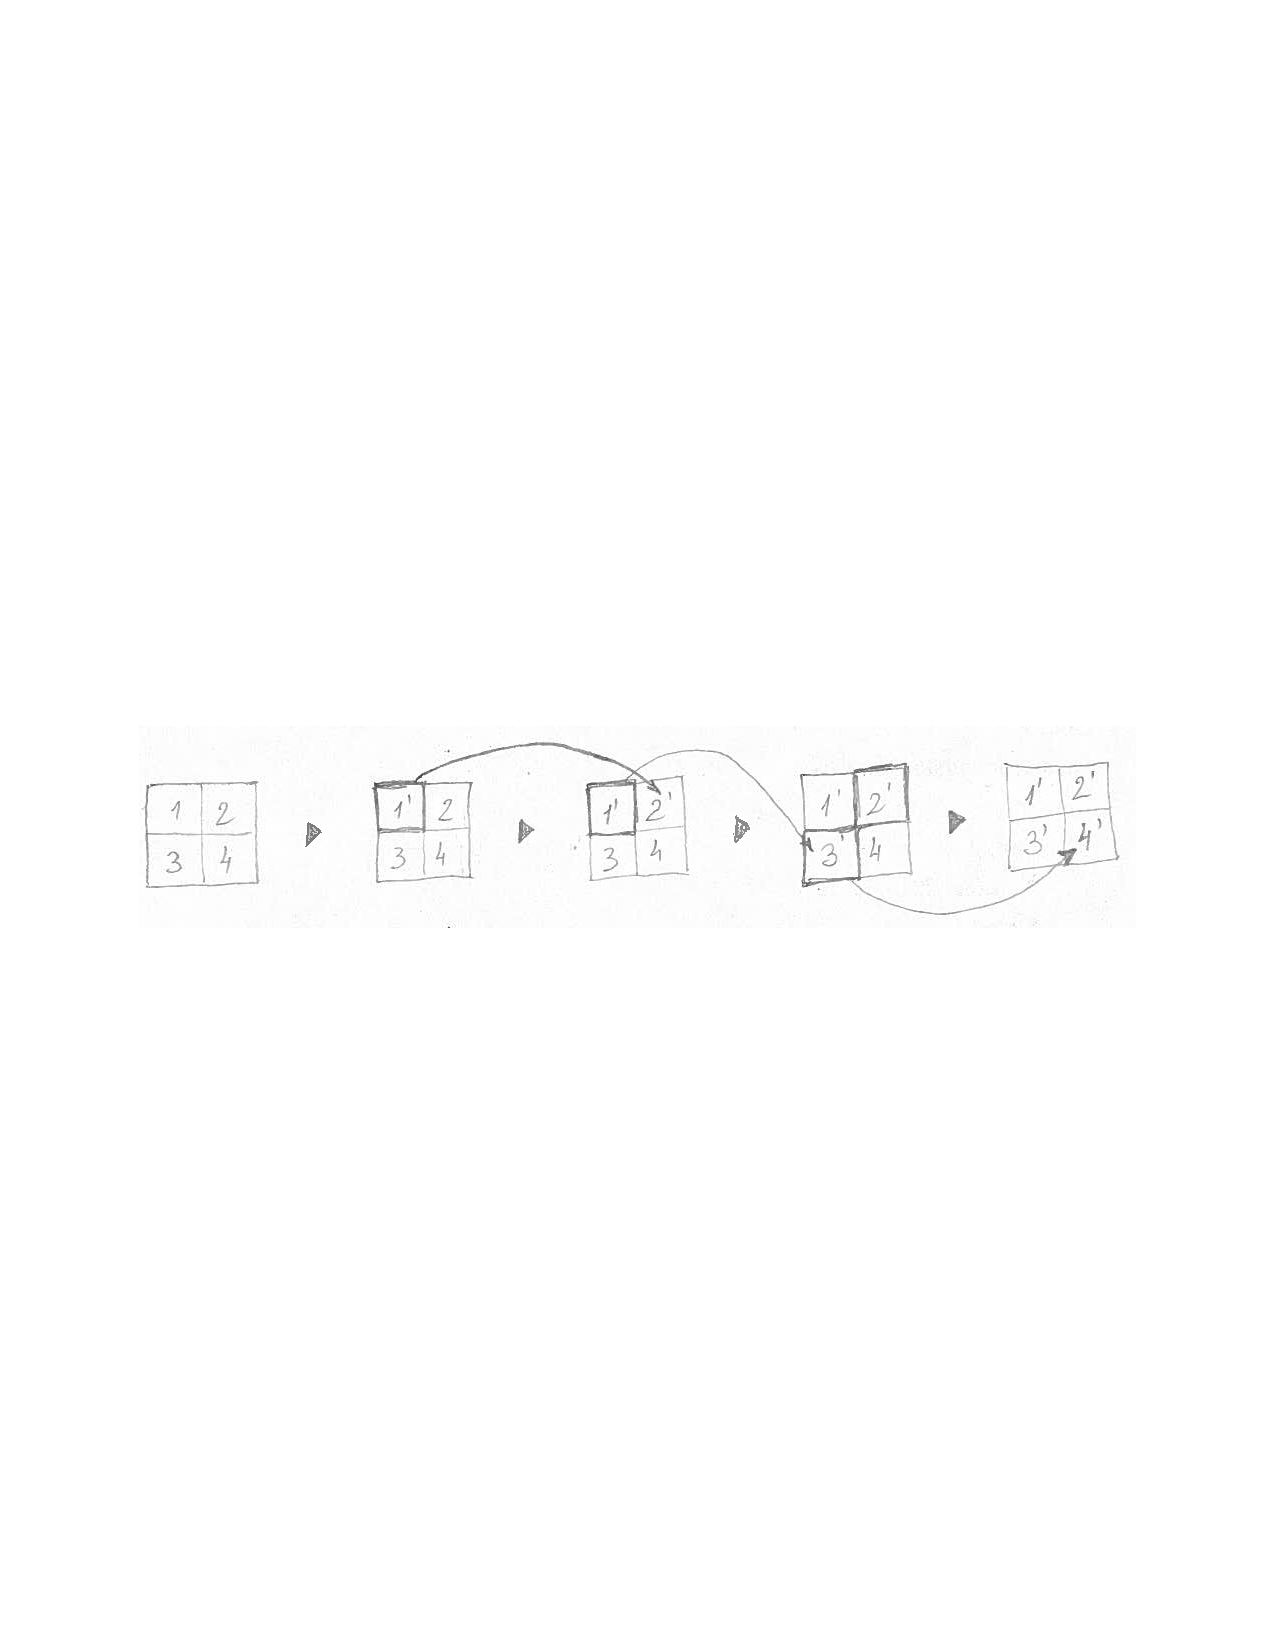
\includegraphics[width=.47\textwidth]{img/gap-stratify1}
\caption[caption]{\label{intro:chain}
  Stratified computation for Simplified Arbiter. \\[.2em]
  Thick borders indicate the region that is read at each step.}
\end{figure}


